\section{Auswertung}
\label{sec:Auswertung}
\subsection{Bestimmung des Materials der Stäbe}
\label{sec:Material}
Mit den aus \ref{sec:Stäbe} bekannten Abmessungen ergeben sich die Dichten $\rho$ der Stäbe mittels
\begin{equation}
  \rho = \frac{m}{V} = \frac{m}{Al}
\end{equation}
und
\begin{equation}
  A_r = \pi r^2
\end{equation}
bzw
\begin{equation}
  A_q = a^2
\end{equation}
zu $\rho_r =8397 \, \symup{\frac{kg}{m^3}}$  bzw. $\rho_q = 8373 \, \symup{\frac{kg}{m^3}}$. Messing CuZnPb3 beispielsweise besitzt eine Dichte von $\rho_{Messing} = 8470 \, \symup{ \frac{kg}{m^3}}$ und einem Elastizitätsmodul von $E_{Messing} = 9.7 \cdot 10^{10} \, \symup{\frac{N}{m^2}}$ \cite{DKI}. Es wird somit von Messingstäben ausgegangen und als vergleichender Theoriewert $E_{Messing}$ hinzugezogen. Auf qualitativen Vergleich wird jedoch verzichtet, da Messing als Legierung je nach Ausführung enorme Unterschiede in seiner Beschaffenheit aufweisen kann.
\subsection{Einseitige Einspannung}
\label{sec:Einseitig}

\begin{table}
  \centering
  \caption{Auslenkung des runden Stabes bei einseitiger Einspannung}
  \label{tab:einseitig-r}
  \sisetup{round-mode = places , round-precision = 3}
  \begin{tabular}{S S S S}
    \toprule
    {$x/cm$} & {$D_o/mm$} & {$D_m /mm$} & {$\Delta D /mm$}\\
    \midrule
    3.000000000000000000e+0 & 0.000000000000000000e+00 & 0.05000000000000000278e-0 & 0.05000000000000000278e-0\\
    4.000000000000000000e+0 & 0.000000000000000000e+00 & 0.04200000000000000261e-0 & 0.04200000000000000261e-0\\
    5.000000000000000000e+0 & 0.04750000000000000056e-0 & 0.05619999999999999996e-0 & 0.008699999999999999400e-0\\
    6.000000000000000000e+0 & 0.05500000000000000028e-0 & 0.1100000000000000006e-0 & 0.05500000000000000028e-0\\
    7.000000000000000000e+0 & 0.06500000000000000222e-0 & 0.1680000000000000104e-0 & 0.1030000000000000082e-0\\
    8.000000000000000000e+0 & 0.1000000000000000056e-0  & 0.2250000000000000056e-0 & 0.1250000000000000000e-0\\
    9.000000000000000000e+0 & 0.1549999999999999989e-0 & 0.2909999999999999809e-0 & 0.1359999999999999820e-0\\
    10.00000000000000000e+0 & 0.1799999999999999933e-0 & 0.3549999999999999822e-0 & 0.1749999999999999889e-0\\
    11.00000000000000000e+0 & 0.2179999999999999993e-0 & 0.4199999999999999845e-0 & 0.2019999999999999851e-0\\
    12.00000000000000000e+0 & 0.2780000000000000249e-0 & 0.4899999999999999911e-0 & 0.2119999999999999662e-0\\
    13.00000000000000000e+0 & 0.3175000000000000044e-0 & 0.5819999999999999618e-0 & 0.2644999999999999574e-0\\
    14.00000000000000000e+0 & 0.3300000000000000155e-0 & 0.6600000000000000311e-0 & 0.3300000000000000155e-0\\
    15.00000000000000000e+0 & 0.3699999999999999956e-0 & 0.7099999999999999645e-0 & 0.3399999999999999689e-0\\
    16.00000000000000000e+0 & 0.4249999999999999889e-0 & 0.8000000000000000444e-0 & 0.3750000000000000555e-0\\
    17.00000000000000000e+0 & 0.4899999999999999911e-0 & 0.9000000000000000222e-0 & 0.4100000000000000311e-0\\
    18.00000000000000000e+0 & 0.5999999999999999778e-0 & 1.040000000000000036e+00 & 0.4400000000000000577e-0\\
    19.00000000000000000e+0 & 0.6899999999999999467e-0 & 1.165000000000000036e+00 & 0.4750000000000000888e-0\\
    20.00000000000000000e+0 & 0.7349999999999999867e-0 & 1.268000000000000016e+00 & 0.5330000000000000293e-0\\
    21.00000000000000000e+0 & 0.8100000000000000533e-0 & 1.381000000000000005e+00 & 0.5709999999999999520e-0\\
    22.00000000000000000e+0 & 0.9280000000000000471e-0 & 1.550000000000000044e+00 & 0.6219999999999999973e-0\\
    23.00000000000000000e+0 & 1.000000000000000000e+00 & 1.705000000000000071e+00 & 0.7050000000000000711e-0\\
    24.00000000000000000e+0 & 1.070000000000000062e+00 & 1.784999999999999920e+00 & 0.7149999999999998579e-0\\
    25.00000000000000000e+0 & 1.129999999999999893e+00 & 1.919999999999999929e+00 & 0.7900000000000000355e-0\\
    26.00000000000000000e+0 & 1.237500000000000044e+00 & 2.250000000000000000e+00 & 1.012499999999999956e+00\\
    27.00000000000000000e+0 & 1.314999999999999947e+00 & 2.169999999999999929e+00 & 0.8549999999999999822e-0\\
    28.00000000000000000e+0 & 1.385000000000000009e+00 & 2.270000000000000018e+00 & 0.8850000000000000089e-0\\
    29.00000000000000000e+0 & 1.449999999999999956e+00 & 2.399999999999999911e+00 & 0.9499999999999999556e-0\\
    30.00000000000000000e+0 & 1.540000000000000036e+00 & 2.555000000000000160e+00 & 1.015000000000000124e+00\\
    31.00000000000000000e+0 & 1.622999999999999998e+00 & 2.750000000000000000e+00 & 1.127000000000000002e+00\\
    32.00000000000000000e+0 & 1.449999999999999956e+00 & 2.825000000000000178e+00 & 1.375000000000000222e+00\\
    33.00000000000000000e+0 & 1.792000000000000037e+00 & 2.959999999999999964e+00 & 1.167999999999999927e+00\\
    34.00000000000000000e+0 & 1.860000000000000098e+00 & 3.084999999999999964e+00 & 1.224999999999999867e+00\\
    35.00000000000000000e+0 & 1.918                    & 3.250000000000000000e+00 & 1.332000000000000073e+00\\
    36.00000000000000000e+0 & 2.01                     & 3.359999999999999876e+00 & 1.350000000000000089e+00\\
    37.00000000000000000e+0 & 2.060000000000000053e+00 & 3.500000000000000000e+00 & 1.439999999999999947e+00\\
    38.00000000000000000e+0 & 2.085                    & 3.620000000000000107e+00 & 1.535000000000000142e+00\\
    39.00000000000000000e+0 & 2.19e+00                 & 3.785000000000000142e+00 & 1.595000000000000195e+00\\
    40.00000000000000000e+0 & 2.270000000000000018e+00 & 3.904999999999999805e+00 & 1.634999999999999787e+00\\
    41.00000000000000000e+0 & 2.350000000000000089e+00 & 4.044999999999999929e+00 & 1.694999999999999840e+00\\
    42.00000000000000000e+0 & 2.635e+00                & 4.174999999999999822e+00 & 1.540000000000000036e+00\\
    43.00000000000000000e+0 & 2.540000000000000036e+00 & 4.339999999999999858e+00 & 1.799999999999999822e+00\\
    44.00000000000000000e+0 & 2.625000000000000000e+00 & 4.549999999999999822e+00 & 1.924999999999999822e+00\\
    45.00000000000000000e+0 & 2.735                    & 4.629999999999999893e+00 & 1.895000000000000018e+00\\
    46.00000000000000000e+0 & 2.82                     & 4.834999999999999964e+00 & 2.015000000000000124e+00\\
    47.00000000000000000e+0 & 2.910000000000000142e+00 & 5.019999999999999574e+00 & 2.109999999999999432e+00\\
    48.00000000000000000e+0 & 2.985                    & 5.184999999999999609e+00 & 2.199999999999999734e+00\\
    49.00000000000000000e+0 & 3.120000000000000107e+00 & 5.290000000000000036e+00 & 2.169999999999999929e+00\\
    \bottomrule
  \end{tabular}
\end{table}

\begin{table}
  \centering
  \caption{Auslenkung des eckigen Stabes bei einseitiger Einspannung}
  \label{tab:einseitig-q}
  \sisetup{round-mode = places , round-precision = 3}
  \begin{tabular}{S S S S}
    \toprule
    {$x/cm$} & {$D_o/mm$} & {$D_m /mm$} & {$\Delta D /mm$}\\
    \midrule
    3.000000000000000000e+00 & 0.000000000000000000e+00 & 0.02000000000000000042e-0 & 0.02000000000000000042e-0\\
    5.000000000000000000e+00 & -0.04000000000000000083e-0 & -0.02000000000000000042e-0 & 0.02000000000000000042e-0\\
    7.000000000000000000e+00 & -0.07000000000000000666e-0 & 0.08000000000000000167e-0 & 0.1500000000000000222e-0\\
    9.000000000000000000e+00 & -0.05500000000000000028e-0 & 0.1900000000000000022e-0 & 0.2449999999999999956e-0\\
    11.00000000000000000e+0 & -0.01000000000000000021e-0 & 0.3300000000000000155e-0 & 0.3400000000000000244e-0\\
    13.00000000000000000e+0 & 0.02000000000000000042e-0 & 0.5150000000000000133e-0 & 0.4949999999999999956e-0\\
    15.00000000000000000e+0 & .05999999999999999778e-0 & 0.6680000000000000382e-0 & 0.6080000000000000959e-0\\
    17.00000000000000000e+0 & 0.1199999999999999956e-0 & 0.9120000000000000329e-0 & 0.7920000000000000373e-0\\
    19.00000000000000000e+0 & 0.2949999999999999845e-0 & 1.270000000000000018e+00 & 0.9750000000000000888e-0\\
    21.00000000000000000e+0 & 0.4299999999999999933e-0 & 1.580000000000000071e+00 & 1.150000000000000133e+00\\
    23.00000000000000000e+0 & 0.5699999999999999512e-0 & 1.899999999999999911e+00 & 1.330000000000000071e+00\\
    25.00000000000000000e+0 & 0.6830000000000000515e-0 & 2.205000000000000071e+00 & 1.522000000000000020e+00\\
    27.00000000000000000e+0 & 0.7950000000000000400e-0 & 2.555000000000000160e+00 & 1.760000000000000231e+00\\
    29.00000000000000000e+0 & 0.9200000000000000400e-0 & 2.915000000000000036e+00 & 1.995000000000000107e+00\\
    31.00000000000000000e+0 & 1.070000000000000062e+00 & 3.310000000000000053e+00 & 2.240000000000000213e+00\\
    33.00000000000000000e+0 & 1.235000000000000098e+00 & 3.714999999999999858e+00 & 2.479999999999999538e+00\\
    35.00000000000000000e+0 & 1.387999999999999901e+00 & 4.125000000000000000e+00 & 2.737000000000000099e+00\\
    37.00000000000000000e+0 & 1.495000000000000107e+00 & 4.509999999999999787e+00 & 3.014999999999999680e+00\\
    39.00000000000000000e+0 & 1.705000000000000071e+00 & 4.974999999999999645e+00 & 3.269999999999999574e+00\\
    41.00000000000000000e+0 & 1.879999999999999893e+00 & 5.419999999999999929e+00 & 3.540000000000000036e+00\\
    43.00000000000000000e+0 & 2.009999999999999787e+00 & 5.879999999999999893e+00 & 3.870000000000000107e+00\\
    45.00000000000000000e+0 & 2.169999999999999929e+00 & 6.309999999999999609e+00 & 4.139999999999999680e+00\\
    47.00000000000000000e+0 & 2.365000000000000213e+00 & 6.820000000000000284e+00 & 4.455000000000000071e+00\\
    49.00000000000000000e+0 & 2.595000000000000195e+00 & 7.250000000000000000e+00 & 4.654999999999999361e+00\\
    \bottomrule
  \end{tabular}
\end{table}
\FloatBarrier

Für den runden Stab wurde eine Belastungsmasse von $m_1 = 238.9 \, \symup{g}$ gewählt, für den eckigen $m_2 = 767.5\, \symup{g}$. Ihre Auslenkungen sind in den Tabellen \ref{tab:einseitig-r} und \ref{tab:einseitig-q} aufgelistet. Hierbei bezeichnet $x$ die Position auf dem Stab (Einspannung bei $x = 0$). $D_0$ die Auslenkung im unbelasteten Zustand, $ D_m$ die Auslenkung im belasteten Zustand und $\Delta D$ ihre Differenzen, also die Auslenkung durch die Belastung. Graphisch dargestellt sind die Werte in Abb.\ref{fig:Reihe1} bzw. Abb.\ref{fig:Reihe2}.

\begin{figure}
  \centering
  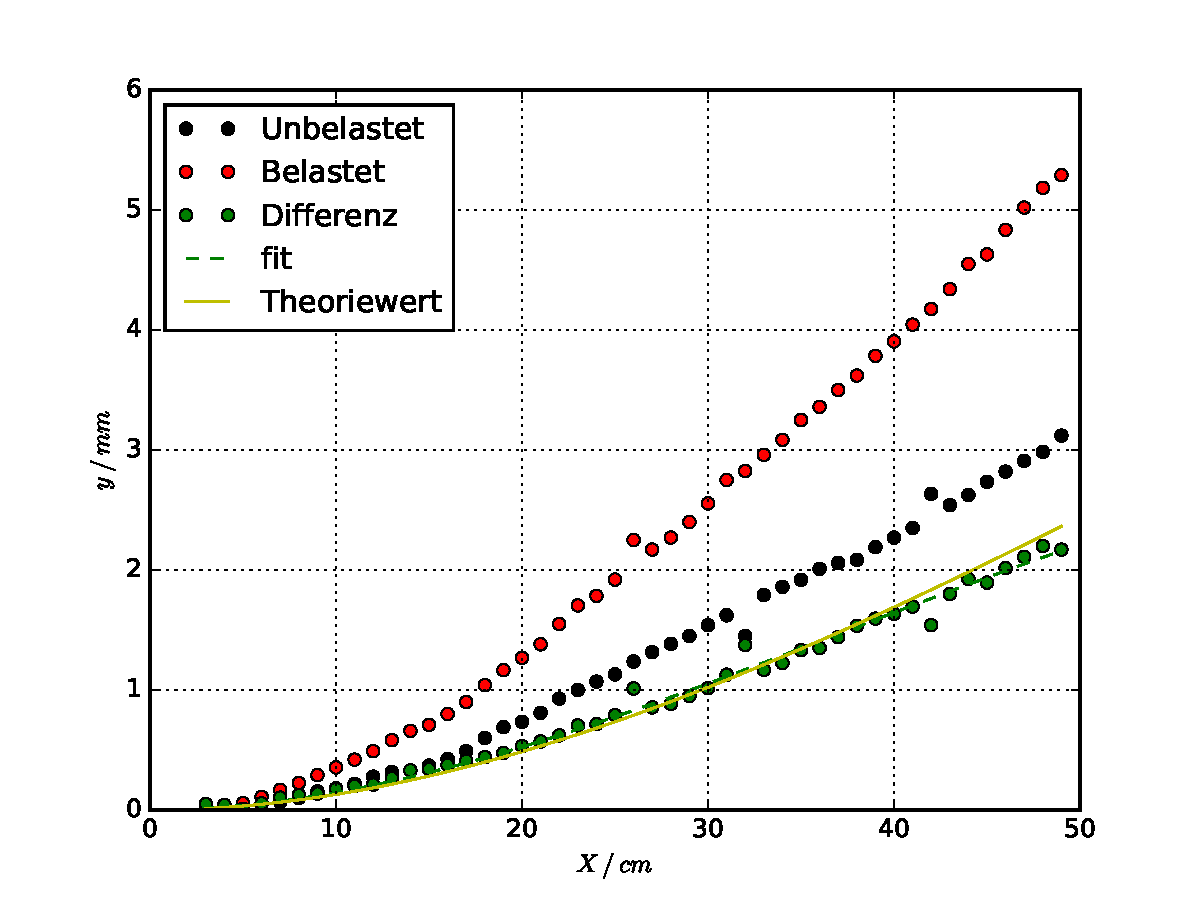
\includegraphics[width = \textwidth]{./Plots/Reihe1.pdf}
  \caption{Auslenkung des runden Stabes, verglichen mit dem Theoriewert.}
  \label{fig:Reihe1}
\end{figure}

\begin{figure}
  \centering
  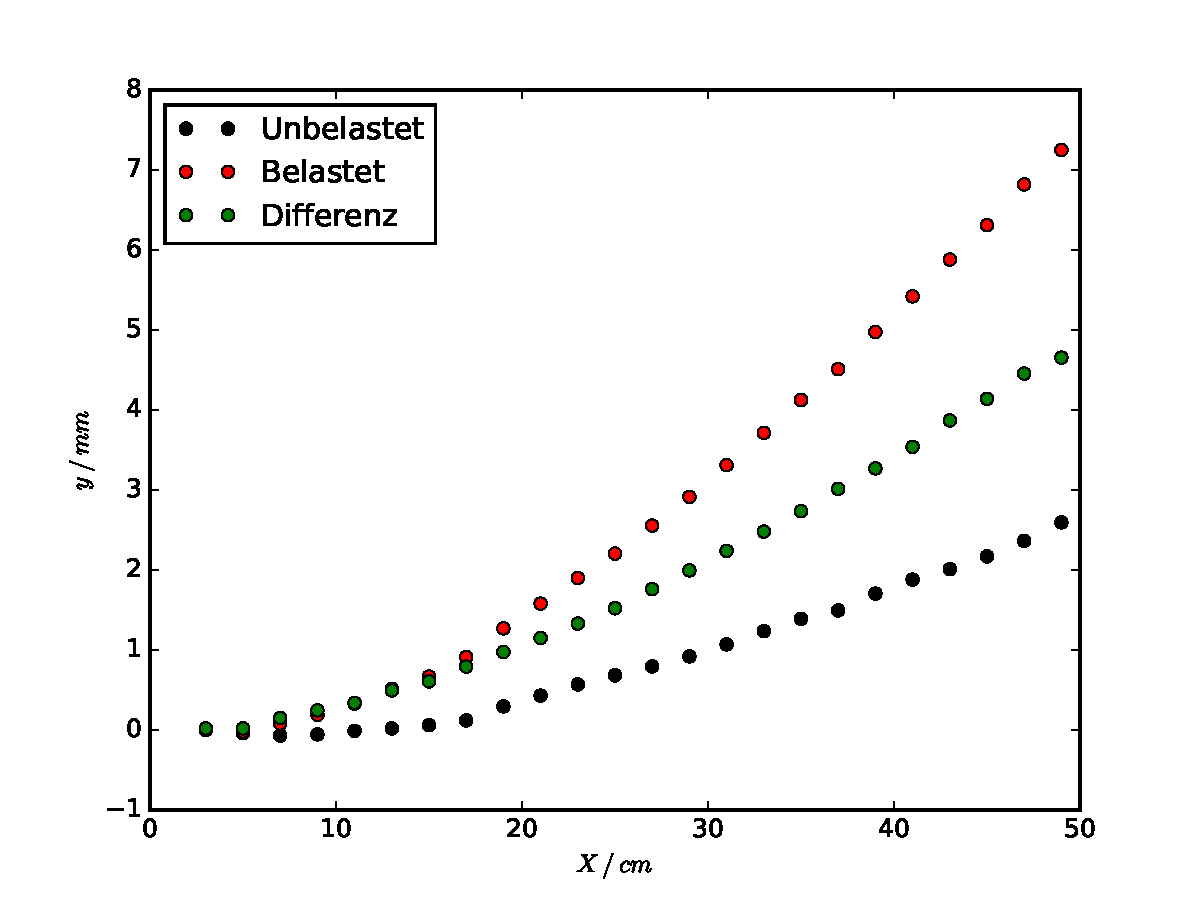
\includegraphics[width = \textwidth]{./Plots/Reihe2.pdf}
  \caption{Auslenkung des eckigen Stabes, verglichen mit dem Theoriewert.}
  \label{fig:Reihe2}
\end{figure}

Die Flächenträgheitsmomente der Stäbe ergeben sich über \eqref{eqn:I} zu
\begin{equation}
  I_r = \int_{-\pi/2}^{\pi/2} \frac{d^4}{8} sin^2(\phi) cos^2(\phi)\symup{d\phi}= \frac{\pi}{64}d^4 = 4.9 \cdot 10^{-10} \, \symup{m^4}
\end{equation}
bzw.
\begin{equation}
  I_q = a \int_{-a/2}^{a/2} y^2 \symup{dy} =\frac{a^4}{12} = 8.3\cdot 10^{-10} \, \symup{m^4}
\end{equation}

Mittels linearer Ausgleichsrechnung ($f = a z +b$ mit $z = Lx^2-x^3/3$) der Auslenkung der Stäbe lässt sich durch \eqref{eqn:D1} der Elastizitätsmodul bestimmen, wobei $E = \frac{F}{2aI}$ gilt, da $b \approx 0$. Die entsprechenden Werte der Parameter lauten:
\begin{align}
  a_r &= \left( 2.1968\pm 0.0324 \right)  \cdot 10^{-2}  \, \symup{\frac{1}{m^2}} \\
  b_r &= \left(7.36 \pm 1.60 \right) \cdot 10^{-5} \, \symup{m}                   \\
  a_q &= \left(4.4922 \pm 0.0027 \right)  \cdot 10^{-2}  \, \symup{\frac{1}{m^2}} \\
  b_r &= \left(5.69 \pm 1.43 \right) \cdot 10^{-5} \, \symup{m}
\end{align}
 Hierraus ergeben sich

\begin{equation*}
  E_r = \left(1.089 \pm 0.004\right)\cdot 10^{11} \, \symup{\frac{N}{m^2}}
\end{equation*}
und
\begin{equation*}
  E_q = \left(1.0097 \pm 0.0013 \right)\cdot 10^{11} \, \symup{\frac{N}{m^2}}.
\end{equation*}



\subsection{Beidseitige Auflage}
\label{sec:Beidseitig}

\begin{table}
  \centering
  \caption{Auslenkung des beidseitig aufgelegten runden Stabes}
  \label{tab:Erb}
  \sisetup{round-mode = places , round-precision = 2}
  \begin{tabular}{S S S S}
    \toprule
    {$x/cm$} & {$D_0 /mm$} & {$D_m / mm$} & {$\Delta D /mm$}\\
    \midrule
    3.000000000000000000e+00 & 0.02999999999999999889e-0 & 0.5649999999999999467e-0 & 0.5349999999999999201e-0\\
    5.000000000000000000e+00 & -0.04000000000000000083e-0 & 0.8649999999999999911e-0 & 0.9050000000000000266e-0\\
    7.000000000000000000e+00 & -0.1000000000000000056e-0 & 1.175000000000000044e+00 & 1.275000000000000133e+00\\
    9.000000000000000000e+00 & -0.1499999999999999944e-0 & 1.495000000000000107e+00 & 1.645000000000000018e+00\\
    11.00000000000000000e+0 & -0.1650000000000000078e-0 & 1.379999999999999893e+00 & 1.544999999999999929e+00\\
    13.00000000000000000e+0 & -0.2250000000000000056e-0 & 2.040000000000000036e+00 & 2.265000000000000124e+00\\
    15.00000000000000000e+0 & -0.3200000000000000067e-0 & 2.270000000000000018e+00 & 2.589999999999999858e+00\\
    17.00000000000000000e+0 & -0.3400000000000000244e-0 & 2.520000000000000018e+00 & 2.859999999999999876e+00\\
    19.00000000000000000e+0 & -0.2999999999999999889e-0 & 2.774999999999999911e+00 & 3.074999999999999734e+00\\
    21.00000000000000000e+0 & -0.3400000000000000244e-0 & 2.950000000000000178e+00 & 3.290000000000000036e+00\\
    23.00000000000000000e+0 & -0.3099999999999999978e-0 & 3.104999999999999982e+00 & 3.415000000000000036e+00\\
    25.00000000000000000e+0 & -0.3499999999999999778e-0 & 3.200000000000000178e+00 & 3.550000000000000266e+00\\
    30.00000000000000000e+0 & 0.7049999999999999600e-0 & 3.600000000000000089e+00 & 2.895000000000000018e+00\\
    32.00000000000000000e+0 & 0.6099999999999999867e-0 & 3.479999999999999982e+00 & 2.870000000000000107e+00\\
    34.00000000000000000e+0 & 0.5699999999999999512e-0 & 3.370000000000000107e+00 & 2.800000000000000266e+00\\
    36.00000000000000000e+0 & 0.5200000000000000178e-0 & 3.180000000000000160e+00 & 2.660000000000000142e+00\\
    38.00000000000000000e+0 & 0.4849999999999999867e-0 & 2.959999999999999964e+00 & 2.475000000000000089e+00\\
    40.00000000000000000e+0 & 0.4299999999999999933e-0 & 2.714999999999999858e+00 & 2.284999999999999698e+00\\
    42.00000000000000000e+0 & 0.3850000000000000089e-0 & 2.439999999999999947e+00 & 2.054999999999999716e+00\\
    44.00000000000000000e+0 & 0.3599999999999999867e-0 & 2.157500000000000195e+00 & 1.797500000000000320e+00\\
    46.00000000000000000e+0 & 0.2999999999999999889e-0 & 1.787500000000000089e+00 & 1.487500000000000044e+00\\
    48.00000000000000000e+0 & 0.2200000000000000011e-0 & 1.419999999999999929e+00 & 1.199999999999999956e+00\\
    50.00000000000000000e+0 & 0.1600000000000000033e-0 & 1.030000000000000027e+00 & 0.8699999999999999956e-0\\
    52.00000000000000000e+0 & 0.9800000000000000377e-0 & 0.6149999999999999911e-0 & 0.5170000000000000151e-0\\
    54.00000000000000000e+0 & 0.000000000000000000e+00 & 0.1900000000000000022e-0 & 0.1900000000000000022e-0\\
    \bottomrule
  \end{tabular}
\end{table}

In diesem Versuchsteil ist die Belastung $m_3 = 4722.5 \, \symup{g}$. Die Auslenkungen des Stabes sind Tabelle \ref{tab:beidseitig} zu entnehmen, die entsprechende Graphik stellt Abb. \ref{fig:Reihe2} dar. In Abb. \ref{fig:Fit} sind die Werte der linken Hälfte des Stabes gemäß \eqref{eqn:D2} linearisiert dargestellt.
Die Berrechnung von $E_r$ erfolgt erneut durch einen linearen Ausgleich ($f = ax +b$), aus dem sich der Elastizitätsmodul aus \eqref{eqn:D2} bestimmen lässt, wobei $E = \frac{F}{48aI}$ gilt, da $b \approx 0$. Es wird hierbei nur mit den Werten der linken Hälfte ($x<27 \, \symup{cm}$) gerechnet, da sich Abb. \ref{fig:Reihe3} entnehmen lässt, dass die Werte der rechten Hälfte eine starke systematische Abweichung aufweisen (siehe Abschnitt \ref{sec:Diskussion}).
\begin{equation*}
  E_{links} = \left(1.01 \pm 0.04 \right)\cdot 10^{11} \, \symup{\frac{N}{m^2}}
\end{equation*}


\begin{figure}
  \centering
  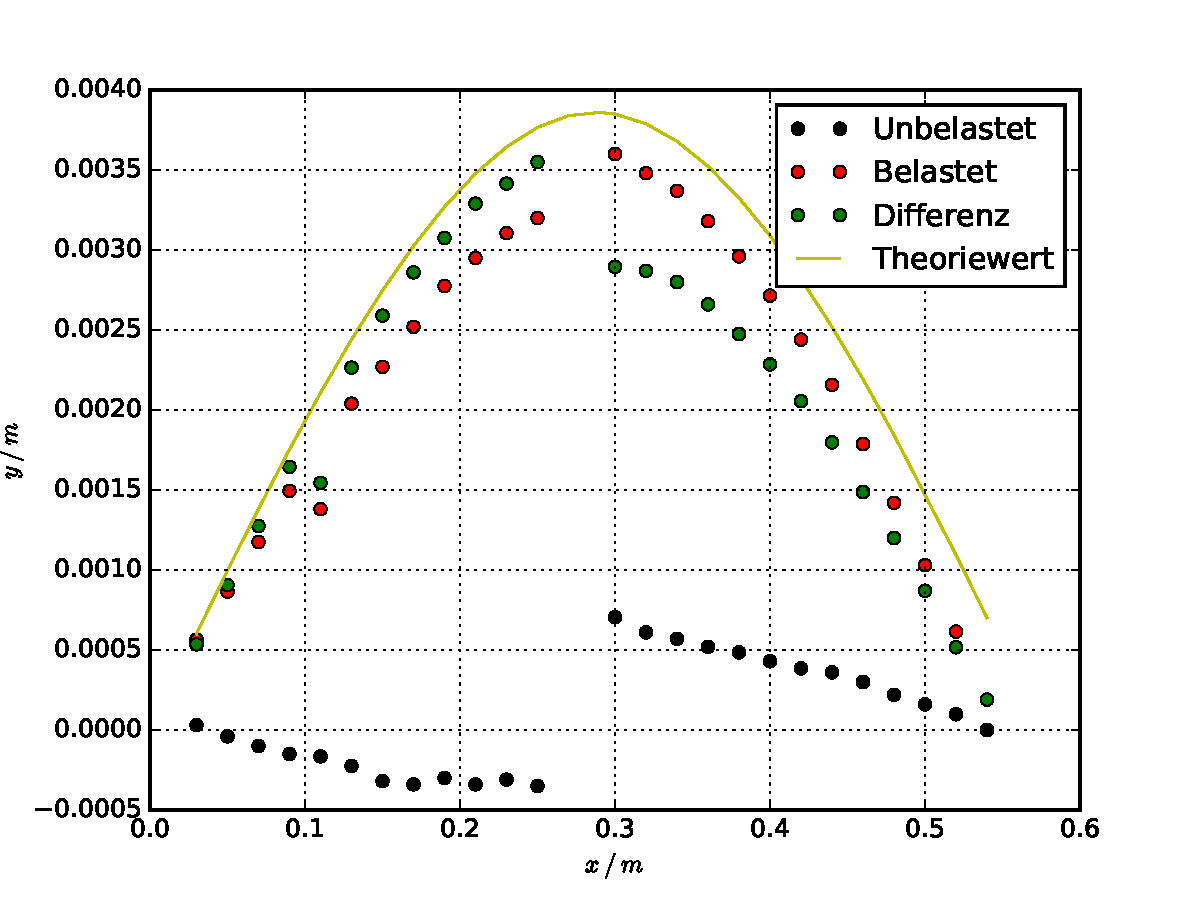
\includegraphics[width = \textwidth]{./Plots/Reihe3.pdf}
  \caption{Auslenkung des runden Stabes bei beidseitiger Auflage, verglichen mit dem Theoriewert.}
  \label{fig:Reihe3}
\end{figure}

\begin{figure}
  \centering
  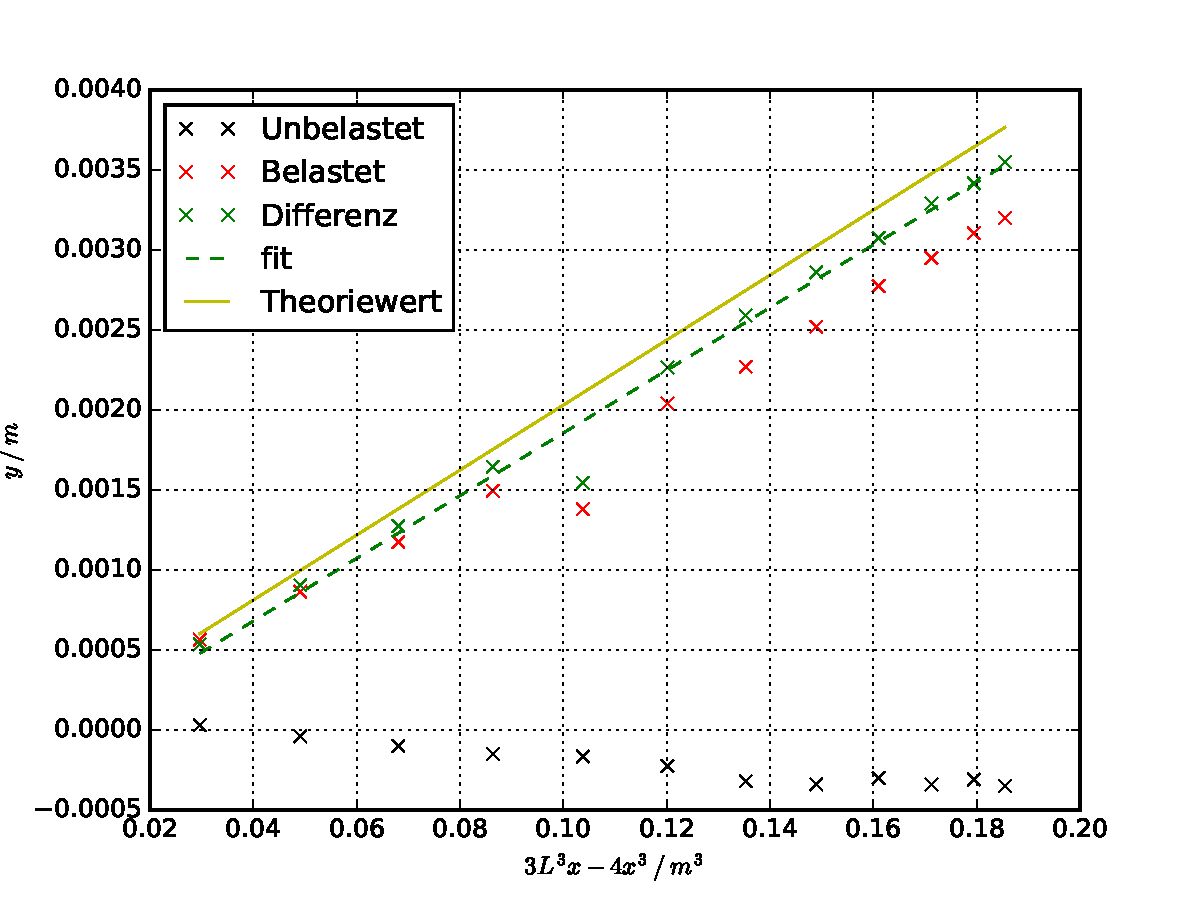
\includegraphics[width = \textwidth]{./Plots/beidseitigFit.pdf}
  \caption{Auslenkung der linken Hälfte des runden Stabes bei beidseitiger Auflage, verglichen mit dem Theoriewert sowie linearem Ausgleich.}
  \label{fig:Fit}
\end{figure}
